\chapter{Background}
\label{cha:background}

\section{Binary Search}
Binary search is a common algorithm for searching through a sequence for a target value.
The algorithm utilises a binary tree for the search.
The algorithm can be described by the following steps, from Knuth \cite{Knuth1971}:
\begin{enumerate}
    \item If the tree has no root node, the search is unsuccessful. 
    The target value is not in the tree, as the tree is empty.
    \item If the root node has the target value, the search is successful.
    The position of the target value is found.
    \item If the target value is smaller than the root value, the left side of the binary tree is explored.
    The algorithm returns to the first step of the procedure.
    This time the tree is the left half of the binary tree, with the new root node being the left child of the previous root node.
    \item If the target value is greater than the root value, the right side of the binary tree is explored.
    The algorithm returns to the first step, but this time the tree is the right subtree of the binary tree.
    The new root node is the right child of the previous root node.
\end{enumerate}
The procedure is illustrated in Figure \ref{fig:binary-search-algorithm}.
The algorithm has a complexity of $O(log_2 n)$, as the search space is in the binary case divided in two after each comparison.
However, the algorithm requires a sorted sequence of values.

\begin{figure}[t!]
    \centering
    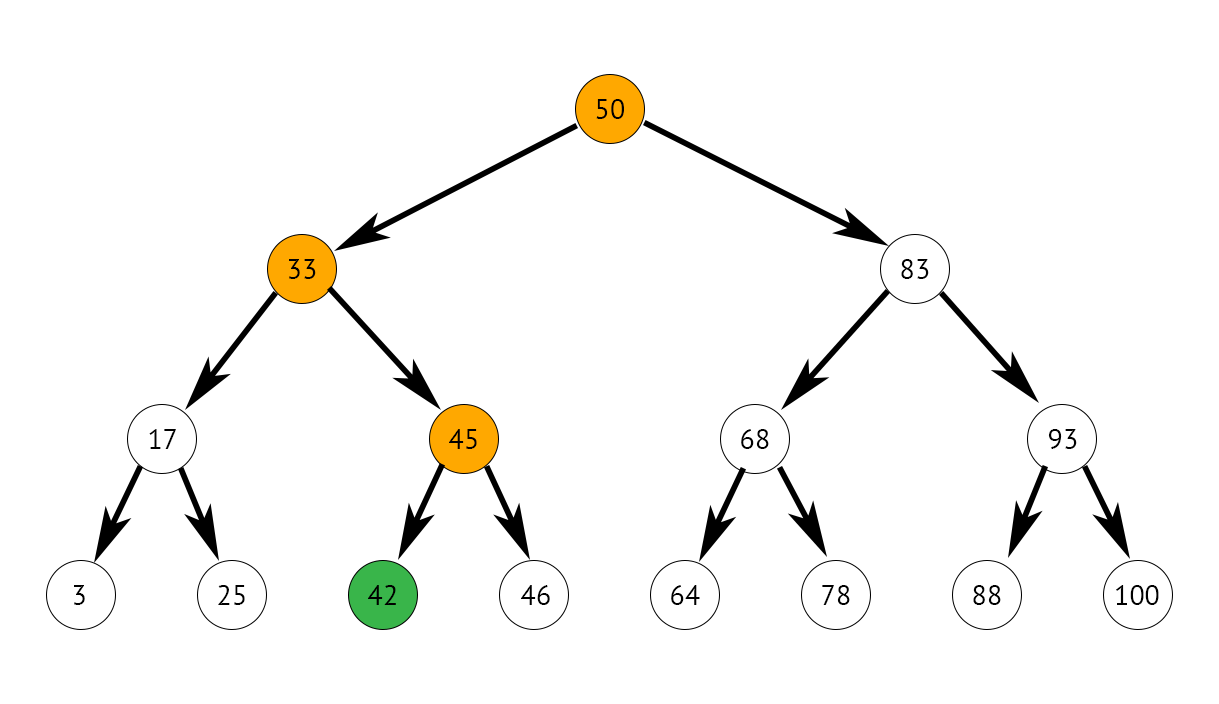
\includegraphics[width=0.9\textwidth]{figures/binary_search_algorithm}
    \caption[Example of a binary search algorithm run]
    {\small Example of a binary search algorithm run.
    The target value is 42.
    First the root node 50 is compared, but as $42 < 50$ the left subtree is explored.
    The new root node is 33 and $42 > 30$, so the right subtree is explored.
    The new root node is 45 and $42 < 45$.
    The algorithm should search the left subtree, which in this case only consists of one node, with the target value.
    The search is successful.}
    \label{fig:binary-search-algorithm}
\end{figure}

\section{Gaussian Processes}
Gaussian processes \cite{Rasmussen2006} (GPs) are a Bayesian non-parametric approach to modelling.
GPs have throughout the years been proved useful when solving a wide variety of real-world problems in various fields.
Recent examples of GPs being used are in the field of astronomy to infer intrinsic spectra and stellar radial velocities \cite{Czekala2017} or to infer stellar rotation periods \cite{Angus2017}.
GPs have also been successfully used in the field of Biomedical Engineering to develop a real-time algorithm which risk scores ward patients \cite{Alaa2018}.
Finley et al. showed in \cite{Finley2017} how GPs could be used to predict the forest canopy height.
In \cite{8082124}, large-scale GPs are used to improve remote sensing image classification and in \cite{Raissi2017} GPs are used to infer linear equation parameters.
In \cite{NIPS2017_6877}, van der Wilk et al. improve the practical aspects for a convolutional structure in GP in order to improve image detection.
In \cite{Stein2017}, Stein conducts a large-scale spatio-temporal data analysis with models based on GPs and in \cite{Dong2017}, Dong et al. perform continuous-time trajectory estimation using GPs.

\subsection{Definition}

Definition \ref{def:gaussian-process} is the formal definition of a GP given by Rasmussen et al. in \cite{Rasmussen2006}.
\begin{definition} \label{def:gaussian-process}
    A Gaussian process is a collection of random variables, any infinite number of which have a joint Gaussian distribution.
\end{definition}

A GP is denoted by the equation
\begin{equation} \label{eq:GP-eq1}
    f(x) \sim \mathcal{GP}(m(x), k(x, x')),
\end{equation}

where 
\begin{itemize}
    \item $m(x) = \mathbb{E}[f(x)]$ is the mean function;
    \item $k(x, x') = \mathbb{E}[(f(x) - m(x))(f(x') - m(x'))]$ is the covariance function.
    $x$ and $x'$ are two inputs.
\end{itemize}

A GP is thus completely described by its mean and covariance function, where the mean function is taken to be zero for notational simplicity \cite{Rasmussen2006}.
It can be seen as a probability distribution over functions.
The covariance function can be expressed in the form of a \textit{kernel}, where kernels exhibit different characteristics.
A comparison between common kernels is illustrated in Figure \ref{fig:gp-kernels}.
The approach is Bayesian as \(f(x) \sim \mathcal{GP}\) encodes a prior belief about the unknown $f(\cdot)$.

\begin{figure} [t!]
    \centering
    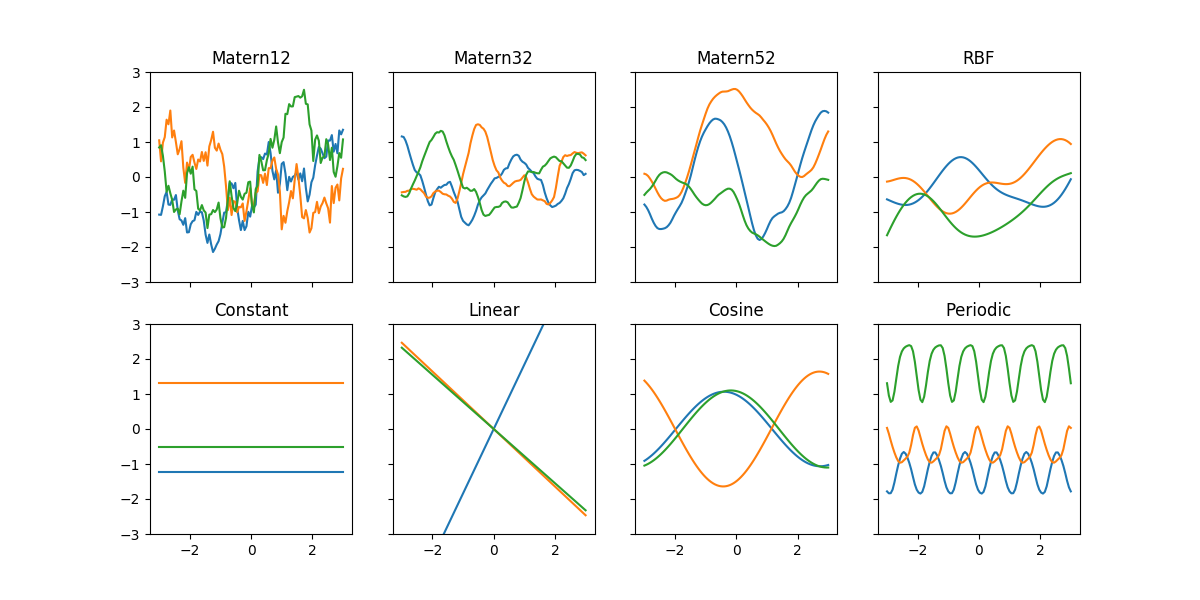
\includegraphics[width=\textwidth]{figures/gp_kernels}
    \caption[Samples from GP priors defined by common covariance functions]
    {\small Samples from GP priors defined by common covariance functions. 
    The functions exhibit different characteristics depending on the choice of kernel.}
    \label{fig:gp-kernels}
\end{figure}

Gaussian process regression (GPR) aims at reconstruct the underlying, unknown $f(\cdot)$ without the observation noise $\epsilon$.
The GPR model is given by
\begin{equation}
    y = f(x) + \epsilon,
\end{equation}
where
\[\epsilon \overset{iid}{\sim} \mathcal{N}(0, \sigma_{noise}^2)\]
and $f(\cdot)$ is a prior.
Here $\epsilon$ represents noisy observations, where $\epsilon$ is assumed to be additive independent identically distributed (iid) Gaussian noise.

The posterior of a GP is also a GP \cite{Rasmussen2006}, with a Gaussian predictive distribution given by the posterior GP evaluated at the new point $x_\star$.
The GP prediction (posterior) is defined by the equation
\begin{equation}
    p(f_\star|x, y, x_\star) \sim \mathcal{GP}(\bar{f}_\star, cov(f_\star)),
\end{equation}
where $\bar{f}_\star$ and $cov(f_\star)$ are given by the equations
\begin{align}
    \bar{f}_\star &= K(x_\star, x)[K(x, x) + \sigma^2_{noise}I]^{-1}y \\
    cov(f_\star) &= K(x_\star, x_\star) - K(x_\star, x)[K(x, x) + \sigma^2_{noise}I]^{-1}K(x,x_\star),
\end{align}
where $K(x_\star, x), K(x, x)$, and $K(x, x_\star)$ each are a covariance (Gram) matrix \cite{Rasmussen2006}.  

\subsection{Related Work}
\section{Combining GPs}
\todo{...}

\subsection{GPflow}
GPflow\footnote{https://gpflow.readthedocs.io/en/latest/index.html} \cite{GPflow2017} is a GP framework for the Python programming language \footnote{https://www.python.org/} using TensorFlow\footnote{https://www.tensorflow.org/}.
It is an open-source software which has its origins from the contributors of GPy\footnote{https://sheffieldml.github.io/GPy/}, another famous framework for implementing GPs in Python.
As GPflow is built upon TensorFlow, it achieves better performance when using GPUs for processing \cite{GPflow2017}.
Building GPflow on top of TensorFlow also allows the benefits of using TensorFlow methods for calculations, e.g., most gradient computations are handled by TensorFlow.

\section{Finite-State Machines}
Finite-state machines (FSM) are well-defined mathematical models which can have numerous representations.
The formal notation used here are from the excellent book "Automata and Computability" by Kozen \cite{Kozen1997}.
A FSM is defined as states with potentially multiple transitions between each state.
The FSM can only be in one given state at any time.

Formally a FSM is given by the structure
\[M = (Q, \Sigma, \delta, s, F),\]
where
\begin{itemize}
    \item Q is a finite set of states.
    \item $\Sigma$ is the input alphabet of the FSM.
    \item $\delta : Q \times \Sigma \rightarrow Q$ is the transition function for the FSM.
    It can intuitively be seen as the function which tells the FSM which state to transition to in response to an input.
    For example, if M is in state $q$ and receives input $x$ it should move to state $\delta(q, x)$.
    \item $s \in Q$ is the start state.
    \item $F \subset Q$; where the elements of $F$ are the final states of the FSM.
\end{itemize}

A FSM can be modelled with various representations \cite{Kozen1997}, e.g, in tabular form, as a transition diagram or as a regular expression.

\section{Exploratory Data Analysis}
Exploratory Data Analysis (EDA) is a broad concept containing various techniques \cite{Anselin1999, Gelman2003, Hoaglin2003, Tukey1977, Velleman1981} for exploring and analysing data.
Early popular techniques include \emph{box plots} and \emph{stem-and-leaf} displays.
A stem-and-leaf plot takes numbers and splits them into two groups.
The first group contains the leading digit(s) and the second group contains the trailing digit(s).
Figure \ref{fig:stem-leaf-plot} is an example of a stem-and-leaf plot with one leading and one trailing digit.
The grouping helps when sorting batches of data and visualising important features, without losing the information of every single data point used \cite{Velleman1981}.

\begin{figure} [h!]
    \centering
    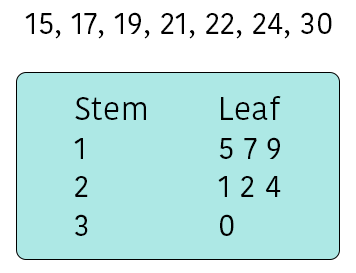
\includegraphics[width=0.33\textwidth]{figures/stem-leaf-plot}
    \caption[Example of a stem-and-leaf plot]
    {\small Example of a stem-and-leaf plot. The numbers above the plot is the input.
    The first digit of the number is the \emph{stem}, the following digits are the \emph{leafs}.}
    \label{fig:stem-leaf-plot}
\end{figure}

EDA can be seen as applying tools and statistics to analyse data in a meaningful way, e.g., it could be applied to the detection of outliers, smoothing the data, and performing a variance analysis \cite{Anselin1999, Hoaglin2003, Tukey1977, Velleman1981}.
EDA can also reveal subtle practical problems with the chosen model that can easily be missed when performing statistical theory analysis of the model \cite{Gelman2003}.

In \cite{Tukey1977}, Tukey describes how EDA can be used to answer research questions such as "What is the age distribution for the Vietnamese population?" and "Are there differences in
the annual household per capita expenditures between the rural and urban populations in Vietnam?".
Tukey uses plots to compare different groups and estimators to quantify the difference.
For example, the sample mean estimator, or the \emph{winsorised} mean can be used \cite{Tukey1977}.
The winsorised mean handles the case where tails of a distribution dominates the value space.  
This would cause the sample mean estimator to poorly reflect on the "typical" data point, as it is skewed by the small tail population \cite{Tukey1977}.

In \cite{Velleman1981}, Velleman et al. present different EDA techniques and highlights four key areas of EDA: displays (plots), residuals, re-expressions and resistance.
Residuals is what remains after data analysis is performed.
Residuals could, for example, be what remains after fitting data to a model (the error of the fit) \cite{Velleman1981}.
Re-expression is the notion of applying mathematical functions to the data.
Re-expressing the data can help with the data analysis \cite{Hoaglin2003, Velleman1981}.
Examples of mathematical functions that can be applied are: logarithm, square root, reciprocal square function or generally raising the data to some power $p$.
Resistance is the concept that outliers should not disproportionately affect the data analysis \cite{Hoaglin2003, Velleman1981}.
For example, the winsorised mean estimator would be less sensitive to localised misbehaviour than the sample mean estimator \cite{Tukey1977}.

Smoothing data is important for many different applications \cite{Bradley1997, Pang2002, Quinlan1992, Velleman1981}.
This can, for example, be done by applying \emph{running median smoothers}.
The running median smoothers go through all the data points in sequence and calculate only the median for the $n$ closest values near each point \cite{Velleman1981}.
Another approach is the \emph{running weighted average} \cite{Velleman1981}.
Instead of taking the median of the $n$ values, the average is calculated.
The average can also be weighted with different functions, like hanning smoothing \cite{Velleman1981}.
The hanning smoothing for three data points is shown in Eq. \ref{eq:hanning}.
It is worth noting that a single outlier will heavily affect the hanning smoothing and that in practice it is common to first apply a running median smoothing to remove outliers \cite{Velleman1981}.

\begin{equation}
    \hat y_t = \frac{1}{4} y_{t-1} + \frac{1}{2} y_t + \frac{1}{4} y_{t + 1} 
    \label{eq:hanning}
\end{equation}